%%%%%####################################################################
% Packages 
%%%%%####################################################################
\documentclass[10pt,compress,xcolor=table]{beamer}

% Packages
\usepackage[utf8]{inputenc}
\usepackage[english]{babel}
\usepackage{csquotes}
\usepackage[T1]{fontenc}
\usepackage{datetime}

% Biblatex
\usepackage{csquotes} % needed for biblatex.
\usepackage{stmaryrd} % for the url symbol in references.
\usepackage[backend=biber, style=authoryear, citestyle=authoryear]{biblatex}
\bibliography{library.bib}
\renewcommand*{\bibfont}{\footnotesize}
\newcommand\enllas{\raise.5pt\hbox{$\boxempty\kern-4.85pt{}^{\nearrow}$}\kern-2pt}

\DeclareFieldFormat{url}{%
  \mkbibacro{URL}\addcolon\space%
  \ifhyperref%
  {\href{#1}{\enllas}}%
  {\url{#1}}}



\usepackage{math}
\usetikzlibrary{positioning}

% Possible options of the package (add/remove below in \usetheme call):
%  - nosectionpages: no pages between sections
%  - flama: use flama font, requires xelatex/lualatex + the font to compile
%  - compressminiframes: put the heading list bullets indications pages on 1 line
\usetheme[compressminiframes]{sorbonne}

% Title page
\title{Von Kármán vortex streets}

%\subtitle{Numerical methods for deterministic and stochastic problems} % optional subtitle
\foottitle{Numerical simulation of von Kármán vortex streets} % optional, printed at the bottom of the slides, by default same as title, can be useful to rewrite when title has a newline for example
\date{\formatdate{08}{03}{2024}}
% Exam Presentation for Out of Equilibrium Systems
\author{V. BALLESTER and J. NÄGERL}
% \institute{LIP6 - Sorbonne Université} % Optional


%%%%####################################################################
%% OWN STUFF
%%%%####################################################################
\usepackage{wasysym} %For clashing sword symbol
\usepackage{textcomp}

%%%%####################################################################
%% BEGIN OF SLIDES
%%%%####################################################################

\begin{document}

\begin{frame}[plain]
  \titlepage
  \setcounter{framenumber}{0}
\end{frame}

%#####################################################################################################################################
\section{Introduction}
\begin{frame}{von Kármán vortex street}
    The \textit{von Kármán vortex street} phenomenon is a classic example of pattern formation in flows behind bodies, characterized by alternating vortices. 

    \begin{figure}
        \centering
        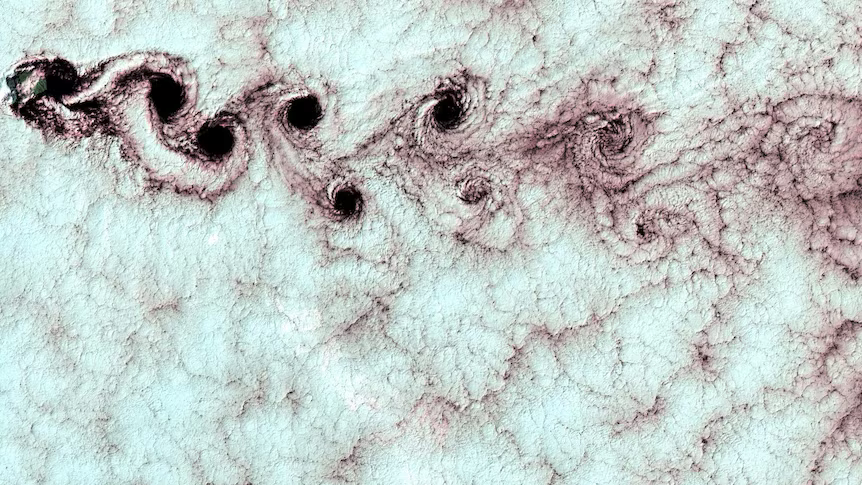
\includegraphics[width=0.6\linewidth]{graphics/example_atmos.png}
        \caption{Atmospheric von Kármán vortex street, showcasing swirling vortices caused by airflow around a mountain (taken from \autocite{wiki})}
        \label{fig:example_vortices}
    \end{figure}
\end{frame}

\begin{frame}{Importance and Objectives}
    \textbf{Why It Matters:}
    \begin{itemize}
        \item Simple phenomenon to study complex flow patterns.
        \item Relevant for cloud formations, and leads to vibrations.
        \item Fundamental example in shape optimization and surface coatings.
    \end{itemize}
    
    \textbf{Project Goals:}
    \begin{itemize}
        \item Simulating von Kármán vortex street in 2D flow using Chorin's method.
        \item Analyzing flow patterns, optimizing for various shapes and configurations.
    \end{itemize}
\end{frame}




%#####################################################################################################################################
\section{Methods}
%Here a lot is missing but for first start I have copied the graphics which content should be included here REFERENCE_numerical. Page 271 main reference \cite{numeric_method_book}
\subsection{Posing the problem} \label{sec: posingProblem}
To simplify our approach we look at a two-dimensional incompressible fluid. In this section we want to pose the problem by introducing the underlying mathematical equations and discuss the boundary conditions.

\subsubsection*{Underlying equations}
In our approach we simplify the problem to a two-dimensional incompressible viscous fluid in a rectangular domain box flowing from one side of the box to the other, encountering an obstacle in its path. The motion of the fluid is described by the \textit{incompressible Navier-Stokes equation}

\begin{align}
  \rho \left( \frac{\partial \textbf{u}}{\partial t}  + \textbf{u} \cdot \nabla \textbf{u} \right)- \mu \Delta \textbf{u}+ \nabla p =0 \label{eq: incompressNS} \\
  \nabla\cdot \textbf{u} = 0 \notag
\end{align}

where $\rho$ is the mass density (assumed constant), $\textbf{u} = (u,v)$ is the fluid velocity with horizontal component $u$ and vertical component $v$, $\mu$ is the dynamic viscosity of the fluid and $p$ is the pressure. The first equation encapsulates the momentum balance within the fluid, incorporating the effects of advection ($\textbf{u} \cdot \nabla \textbf{u}$, velocity interaction and movement), diffusion ($\mu \Delta \textbf{u}$, velocity spreading due to viscosity), and the pressure gradient's influence on the fluid motion ($\nabla p$), whereas the second equation, often termed the \textit{continuity equation}, asserts the incompressibility of the fluid by ensuring the volume conservation within the flow. The equations can be adimensionalized with the following change of variables

\begin{align}
  \Tilde{\textbf{u}} = \frac{\textbf{u}}{U}, \quad \Tilde{p} = \frac{p}{\rho U^2}, \quad \Tilde{\textbf{x}} = \frac{\textbf{x}}{L}, \quad \Tilde{t} = \frac{U}{L}t
\end{align}

where the characteristic velocity $U$ and characteristic length $L$ are used. These quantities represent the typical velocity of the fluid and typical lengthscale. In practice, they are taken to be the inflow velocity and the length of the obstacle in the transverse direction to the flow, respectively. Applying these change of variables to \cref{eq: incompressNS}, we get (dropping the tilde for readability):

\begin{align}
  \frac{\partial \textbf{u}}{\partial t} + \textbf{u} \cdot \nabla \textbf{u} - \frac{1}{\text{Re}} \Delta \textbf{u} + \nabla p = 0 \label{eq:Ns_normalized} \\
  \nabla\cdot\vf{u} = 0 \notag
\end{align}

where the Reynolds number $\Rey := \frac{\rho U L}{\mu}$ is a dimensionless parameter that measures the ratio between the inertia of the flow and the viscosity of it.

\subsubsection*{Boundary conditions}
%The body is first time mentionend here but will be explained later
The domain $\Omega$ is the rectangular box without the obstacle. We call the horizontal direction $x$-direction and the vertical direction $y$-direction. In our study, on the left side a laminar flow is coming into the domain. At the beginning the fluid inside the box is at rest and pressure is null within the domain. At the horizontal walls a slip condition is imposed and a free flow on the right side is assumed. Therefore we obtain as boundary conditions for the walls:

\begin{itemize}
  \item At time $t=0$, the fluid is at rest, and both velocity and pressure are zero.
  \item On the left side, the flow is incoming with a velocity equal to $U \mathbf{e}_x$, and the pressure satisfies the conditions $\frac{\partial p}{\partial x} = 0$.
  \item On the right side of the domain, the flow is free so that $\frac{\partial u}{\partial x} = \frac{\partial v}{\partial x} = 0$ and $p = 0$.
  \item On the horizontal sides, the walls are impenetrable, so that $v = 0$. A slip condition is imposed so that $\frac{\partial u}{\partial y} = 0$ and $\frac{\partial p}{\partial y} = 0$.
\end{itemize}

In order to accurately implement these boundary conditions, we make use of the \textit{ghost cell} method. This technique involves the addition of a layer of cells outside the domain (see \cref{fig: ghostCells}), called \textit{ghost cells}. These cells are used to approximate at second order the values of the velocity and pressure at the boundary for both Dirichlet and Neumann boundary conditions.

\begin{figure}[h]
  \centering
  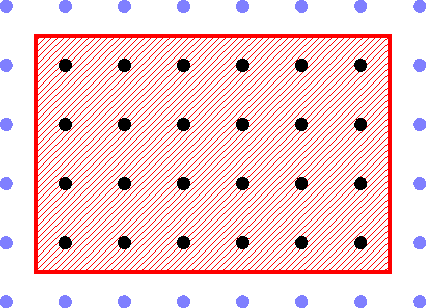
\includegraphics[width=0.5\textwidth]{0_graphics/methods/grid.pdf}
  \caption{The ghost cell method. The domain $\Omega$ is represented in red and the dots represent the grid cells, the black ones being the inner cells and the blue ones, the ghost cells.}
  \label{fig: ghostCells}
\end{figure}

As an example, if $u_{0,j}$ denotes the horizontal component of $\vf{u}$ at the left boundary and height $j$ (counting from 0), then it is approximated by $2U-u_{1,j}$, where $u_{1,j}$ is the horizontal component of $\vf{u}$ at the first cell inside the domain and the same height $j$. A straightforward Taylor expansion around the boundary point (say $u_{1/2,j}$) shows us that indeed this approximation is of second order. Similarly, we obtain values for $v_{0,j}$ and $p_{0,j}$ as

$$
  v_{0,j} = -v_{1,j}, \quad p_{0,j} = p_{1,j}
$$

The other boundaries are treated in the same way, but exchanging the role between $i$ and $j$ and taking into account the different boundary conditions. It should be noted that when computing discrete derivatives, which involve the use of neighbouring cells, the computations are carried out only on the inner cells, which in turn use ghost cells. But the derivatives themselves at ghost cells are never computed.

We discuss now the treatment of the boundary conditions on the object. In general dealing with the object is not an easy task. For simplicity, we model the presence of a solid body within a fluid by enforcing the fluid velocity to be zero inside the object, which correspond to imposing a no-slip condition at the boundary. We can think of it as a direct forcing method, which is a common approach in the literature, and it is based on the idea of adding a forcing term to the Navier-Stokes equations to account for the presence of the object (see \cite{forcing} for more details).
It is very worth-mentioning that the way we integrate the body has an influence on the flow. Especially to study the impacts of coatings or surface structure, our method, is not capable of including these effects, but in our approach we only want to observe the effect, and therefore prioritize simplicity for understanding over complexity for small details in the effect. If the reader is interested in delving deeper into the fluid-structure interactions, including the effects of surface modifications, we recommend consulting works in the field, such as those by Peskin \cite{Peskin1977ImmersedBM} or Schlichting and Gersten \cite{Schlichting2000BoundaryLayerT}.

\subsection{Difference Scheme} \label{sec: diffScheme}
In this section we discuss our numerical solver to integrate \cref{eq:Ns_normalized} together with the boundary conditions presented in above section. To simplify the equations, we use \textit{Chorin's projection method}. It was originally introduced by Alexandre Chorin in 1967 \cite{Chorin1967NumericalNS} as an efficient means of solving the incompressible Navier-Stokes equations.

The idea of the method is to first predict the velocities for the next time step by solving the advection and the diffusion term. With the intermediate velocity field we solve the Poisson equation with a finite difference method (described below). Finally, the \textit{projection step} is preformed, and the velocity field is updated with the new pressure field.

This method is based on the Helmholtz-Hodge decomposition of a vector field $\vf{F}$, which states that any vector field can be decomposed into a sum of a solenoidal (divergence-free) and an irrotational (curl-free) part. In our of fluid dynamics, this means that the velocity field $\vf{u}^*$ can be decomposed into a sum of a solenoidal part $\vf{u}^{n+1}$ and an irrotational part $\nabla p^{n+1}$, where $p^{n+1}$ is the pressure field at time $t^{n+1}$. The projection step is then used to enforce the incompressibility of the velocity field, and to update the velocity field with the new pressure field. 

To ensure that the boundary conditions are met, we impose the conditions for the velocity right before solving the Poisson equation and at the end of each iteration. The boundary conditions for the pressure are imposed after solving the Poisson equation and before correcting the velocities in the projection step.

Next, we provide a summary of the steps in our method. Assuming we know the velocity field at time $t^n$, $\vf{u}^n$, we want to compute the velocity field at time $t^{n+1}$, $\vf{u}^{n+1}$.
\begin{enumerate}
  \item Solve for $\vf{u}^a$ in $\displaystyle  \frac{\vf{u}^a-\vf{u}^n}{\Delta t} + \vf{u}^n \cdot \nabla \vf{u}^n = 0$ using a semi-Lagrangian method.
  \item Solve for $\vf{u}^*$ in $\displaystyle  \frac{\vf{u}^* - \vf{u}^a}{\Delta t} = \frac{1}{\Rey} \laplacian \vf{u}^n$.
  \item Set the boundary conditions for the intermediate velocity field $\vf{u}^*$ and impose the velocity field $\vf{u}^*$ inside the object to be zero (forcing term).
  \item Solve the Poisson equation for the pressure, $\displaystyle \laplacian p^{n+1} = \frac{1}{\Delta t}\nabla \cdot \vf{u}^*$.
  \item Set the boundary conditions for the pressure $p^{n+1}$.
  \item Project the pressure to the intermediate velocity to obtain the new velocity at time $t^{n+1}$, $\displaystyle \vf{u}^{n+1} = \vf{u}^* - \Delta t\nabla p^{n+1}$.
  \item Set the boundary conditions for the velocity field $\vf{u}^{n+1}$.
\end{enumerate}
From these equations, one can easily check that we have:
\begin{align*}
  \frac{\vf{u}^{n+1}-\vf{u}^n}{\Delta t} + \vf{u}^n \cdot \nabla \vf{u}^n - \frac{1}{\Rey} \laplacian \vf{u}^n + \nabla p^{n+1} & = 0 \\
  \nabla \cdot \vf{u}^{n+1}                                                                                                   & = 0
\end{align*}

In the following sections we deepen in how do we compute each of the above steps in our method.

\subsubsection*{Semi-Lagrangian method}
% What is a Semi-Langrangian method
The Semi-Lagrangian (SL) method represents a powerful approach to solving fluid dynamics problems, particularly in the context of advection. Unlike Eulerian methods, which compute changes at fixed points in space, the SL method tracks the motion of fluid parcels. SL methods slightly differ from Lagrangian methods, as the word suggests. The second ones are rarely used in numerical methods because the particle trajectories become chaotic and wildly mixed in a short period of time. However, SL algorithms avoid this problem by \textit{reinitializing} the Lagrangian coordinate system after each time step \cite{Boyd2001ChebyshevFourier}. There are several ways to implement a SL method, and we describe here the one we used in our method. Our goal in this subsection is on solving:

\begin{equation*}
  \frac{\mathrm{D}\vf{u}}{\mathrm{D}t} = \pdv{\vf{u}}{t} + \vf{u} \cdot \nabla \vf{u} = 0
\end{equation*}

The idea is to somehow discretize the material derivative. To do that, if we call $\vf{u}^n$ the current velocity field and $\vf{u}^a$ the velocity field after the advection step, we can write a difference formula as:

\begin{equation*}
  \frac{\vf{u}^a- \vf{u}^n}{\Delta t} + \vf{u}^n \cdot \nabla \vf{u}^n = 0
\end{equation*}

The following discretization for the material derivative is used:

\begin{equation*}
  \frac{\vf{u}(\vf{x}_{i,j},t^{n+1})  - \vf{u}(\vf{x}_{i,j} - \vf{u}(\vf{x}_{i,j},t^n)\Delta t,t^n)}{\Delta t} = 0
\end{equation*}

Here we are approximating the solution along a characteristic line, which generally differs from the actual characteristic associated to the solution at that point, with a constant velocity of $\vf{u}(\vf{x}_{i,j},t^n)$ at each grid point $\vf{x}_{i,j}$.
The reader may rapidly notice that the point $\vf{x}_{i,j} - \vf{u}(\vf{x}_{i,j},t^n)\Delta t$ is not in general in the grid, and thus, we don't have the respective value of the velocity field. To solve this problem, we make use of bilinear interpolation between the four (in 2D) surrounding grid points to the point $\vf{x}_{i,j} - \vf{u}(\vf{x}_{i,j},t^n)\Delta t$. This gives us an approximation of the velocity field at the point $\vf{x}_{i,j} - \vf{u}(\vf{x}_{i,j},t^n)\Delta t$, which in turn provides us with the advected velocity field $\vf{u}^a$.

Furthermore, to improve the accuracy of the method we use the back-and-forth method \cite{backforth}. This method first advects the velocity field using the method described above, and then advects back with opposite velocity $\vf{u}\to -\vf{u}$. With this, we can have an estimate of the error we are comitting when comparing the last result with the initial position. Using this information we can correct the initial velocity field and obtain a more accurate result. The steps are reproduced below. In order to make things more clear, we consider the general case:

\begin{equation*}
  \frac{\mathrm{D}\vf{\psi}}{\mathrm{D}t} = \pdv{\vf{\psi}}{t} + \vf{u} \cdot \nabla \vf{\psi} = 0
\end{equation*}

\begin{enumerate}
  \item Advect the field $\vf\psi^n$ with velocity $\vf{u}$ to obtain $\tilde{\vf{\psi}}^a$.
  \item Advect the field $\vf{\tilde{\psi}}^a$ with velocity $-\vf{u}$ to obtain $\vf{\bar{\psi}}^a$.
  \item Advect the field $\vf{\psi}^n + \frac{1}{2} (\vf{{\psi}}^n - \vf{\bar{\psi}}^a)$ with velocity $\vf{u}$ to obtain $\vf{\psi}^a$.
\end{enumerate}

In our case, the field $\vf\psi$ exactly corresponds to the same velocity field $\vf{u}$. This approach has been proved to be stable and improving considerably the accuracy of the method \cite{backforth}. 

Last but not least, as in all hyperbolic equations, the Courant-Friedrichs-Lewy (CFL) condition must be satisfied. This condition states that the time step $\Delta t$ must be chosen such that the real solution propagates at most at the same speed as the numerical solution. Thus, since we are using an explicit scheme we must impose a CFL of

$$|u|_{\text{max}} \frac{\Delta t}{\Delta x} +|v|_{\text{max}} \frac{\Delta t}{\Delta y}\leq 1$$

\subsubsection*{Diffusion term}
As a second step we add diffusion using a second order central differences. The diffusion term is given by:

\begin{equation*}
  \frac{\vf{u}^* - \vf{u}^a}{\Delta t} = \frac{1}{\Rey} \laplacian \vf{u}^n
\end{equation*}

Once discretized we get for each $i$, $j$ in the grid:

\begin{equation*}
  \vf{u}^*_{i,j} = \vf{u}^a_{i,j} + \frac{\Delta t}{\Rey}\left( \frac{\vf{u}^n_{i+1,j} - 2\vf{u}^n_{i,j} + \vf{u}^n_{i-1,j}}{{(\Delta x)}^2} + \frac{\vf{u}^n_{i,j+1} - 2\vf{u}^n_{i,j} + \vf{u}^n_{i,j-1}}{{(\Delta y)}^2}\right)
\end{equation*}

We write concisely the discretization in vector form, but in practice we do it for each component of the velocity field separately.

\subsubsection*{Solving for the Poisson equation}\label{sec: solvingPoisson}
There are several efficient ways to compute the solution of the general Poisson equation $\Delta p = f$. In our case, we have to equip this equation with the boundary conditions $\partial_{\vf{n}}p=0$ on the left, top and bottom boundaries, and $p=0$ on the right boundary. We use a finite difference method to solve this equation with a 5-point stencil to approximate the Laplacian operator. The 5-point stencil is given by:

\begin{equation*}
  \laplacian p_{i,j} = \frac{p_{i+1,j} - 2 p_{i,j} + p_{i-1,j}}{{(\Delta x)}^2} + \frac{p_{i,j+1} - 2 p_{i,j} + p_{i,j-1}}{{(\Delta y)}^2}
\end{equation*}

If we set $\vf{p}:=(p_{1,1}, p_{1,2}, \ldots, p_{1,n_y}, p_{2,1}, p_{2,2}, \ldots, p_{2,n_y},\ldots, p_{n_x,1},p_{n_x,2},\ldots p_{n_x,n_y})$, we can write our problem in matrix form as $\vf{A}\vf{p}=\vf{f}$, where $\vf{f}$ contains the discrete values at the grid points of the right-hand side of the Poisson equation in the same order as $\vf{p}$, and $\vf{A}$ is a matrix that contains the coefficients of the discrete Laplacian. To describe how we can build the matrix $\vf{A}$, let $\vf{A}=\vf{X} + \vf{Y}$, where $\vf{X}$ and $\vf{Y}$ denote the matrices that contain the coefficients of the Laplacian operator in the $x$ and $y$ directions, respectively. We can write $\vf{X}$ and $\vf{Y}$ as:

\begin{equation*}
  \vf{X} = \begin{pmatrix}
    -\vf{I}_{n_y} & \vf{I}_{n_y}   & \vf{0}         & \cdots       & \cdots         & \vf{0}         \\
    \vf{I}_{n_y}  & -2\vf{I}_{n_y} & \vf{I}_{n_y}   & \ddots       &                & \vdots         \\
    \vf{0}        & \vf{I}_{n_y}   & -2\vf{I}_{n_y} & \vf{I}_{n_y} & \ddots         & \vdots         \\
    \vdots        & \ddots         & \ddots         & \ddots       & \ddots         & \vf{0}         \\
    \vdots        &                & \ddots         & \vf{I}_{n_y} & -2\vf{I}_{n_y} & \vf{I}_{n_y}  \\
    \vf{0}        & \cdots         & \cdots         & \vf{0}       & \vf{I}_{n_y}   & -3\vf{I}_{n_y} \\
  \end{pmatrix}\quad
  \vf{Y} = \begin{pmatrix}
    \vf{B} & \vf{0} & \cdots & \vf{0} \\
    \vf{0} & \vf{B} & \ddots & \vdots \\
    \vdots & \ddots & \ddots & \vf{0} \\
    \vf{0} & \cdots & \vf{0} & \vf{B} \\
  \end{pmatrix}
\end{equation*}

with

$$
  \vf{B} = \begin{pmatrix}
    -1     & 1      & 0      & \cdots & 0      \\
    1      & -2     & 1      & \ddots & \vdots \\
    0      & \ddots & \ddots & \ddots & 0      \\
    \vdots & \ddots & 1      & -2     & 1      \\
    0      & \cdots & 0      & 1      & -1     \\
  \end{pmatrix}\in\mathcal{M}_{n_y}(\mathbb{R})
$$

Both $\vf{X}$ and $\vf{Y}$ are block matrices, composed of $n_x$ matrices in each row and column of size $n_y\times n_y$ each, which results in a matrix of size $n_xn_y\times n_xn_y$. 
The boundary conditions (using ghost cells) on the pressure are applied at both the first and last block rows of $\vf{X}$ and the first and last rows of $\vf{B}$.

In order to solve the resulting system, we use the Cholesky decomposition, which requires the matrix to be symmetric and positive definite. The matrix $\vf{A}$ is symmetric, but it is not positive definite. In fact, it can be seen that it is negative definite. Thus, in our case, we solve the equivalent system $-\vf{A} \vf{p} = -\vf{f}$.


\subsubsection*{Updating velocities}

As a final step, we compute the gradient of the pressure field and update the velocity field. The gradient of the pressure field is computed using a 2nd order central differences scheme. The update of the velocity field is given by:

\begin{equation*}
  \vf{u}_{i,j}^{n+1} = \vf{u}_{i,j}^* - \Delta t \left(
  \frac{p_{i+1,j}^{n} - p_{i,j}^{n}}{\Delta x}, \frac{p_{i,j+1}^{n} - p_{i,j}^{n}}{\Delta y}
  \right)
\end{equation*}


%#####################################################################################################################################
\section{Numerical Results}
\begin{frame}{Observing von Kármán Vortex Street}
    \textbf{Setup:}
    \begin{itemize}
        \item Flow with $\Rey = 500$ ($ \Leftrightarrow\, U = 0.03012$).
        \item Simulation domain: $\dd{x} = \dd{y} = 0.01 $ with a $500 \times 100$ grid.
        \item Circular obstacle with radius $r = 0.125$ initiates flow.
    \end{itemize}
    \vspace{-0.25cm}
    \begin{figure}
        \centering
        \hspace*{0.3cm}
        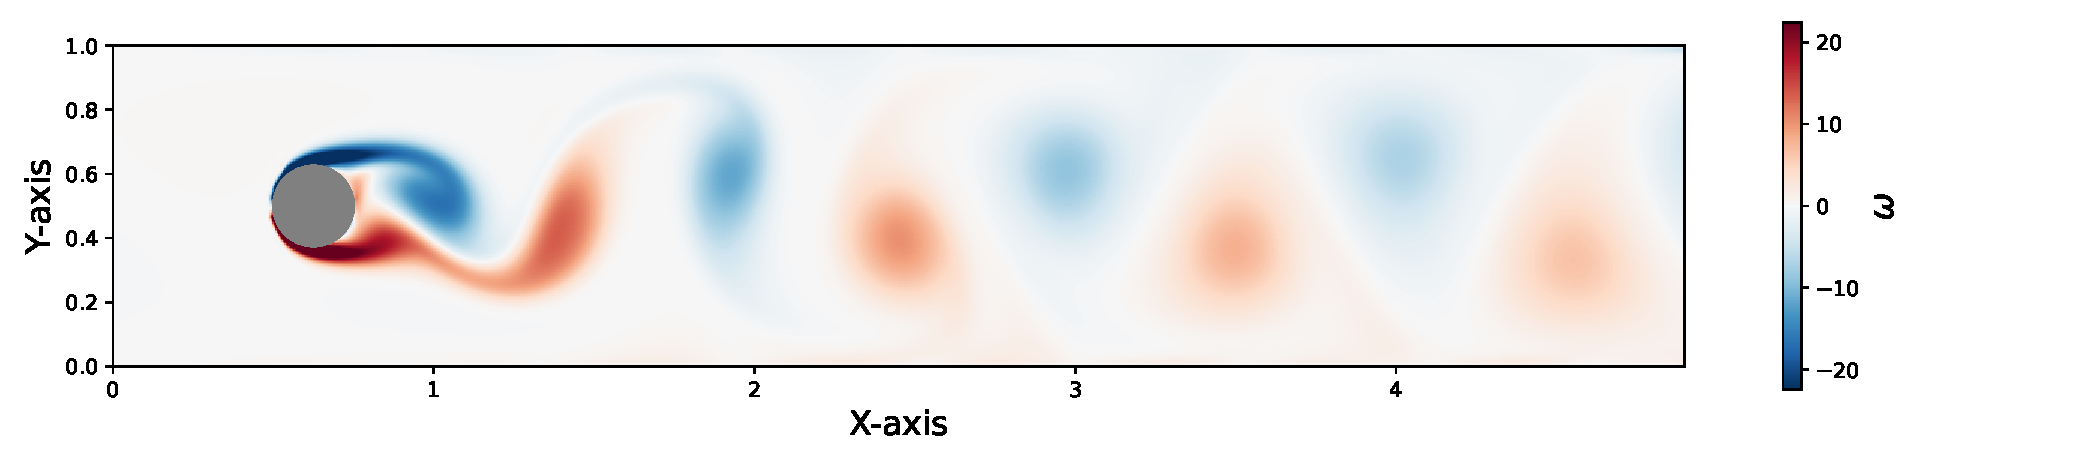
\includegraphics[width=1.1\linewidth]{graphics/numeric/vor_25_sim.pdf}
        \caption{Vorticity $\omega = \nabla \times \vf{u}$ highlighting alternating vortices}
        \label{fig: first_obs}
    \end{figure}
    \vspace{-0.25cm}
    \textbf{Obervations:}
    \begin{itemize}
        \item Laminar front with $u = 1$
        \item Von Kármán vortex street and periodic pattern formation
    \end{itemize}
\end{frame}

\begin{frame}{Influence of Reynolds Number on Flow Dynamics}
    \begin{itemize}
        \item The Reynolds number dictates flow behavior in fluid dynamics.
        \item At a critical $\Rey \approx 175$, flow transitions from laminar to unstable, eventually forming a von Kármán vortex street.
    \end{itemize}
    \vspace{-0.25cm}
        
    \begin{figure}
        \centering
        \hspace*{0.3cm}
        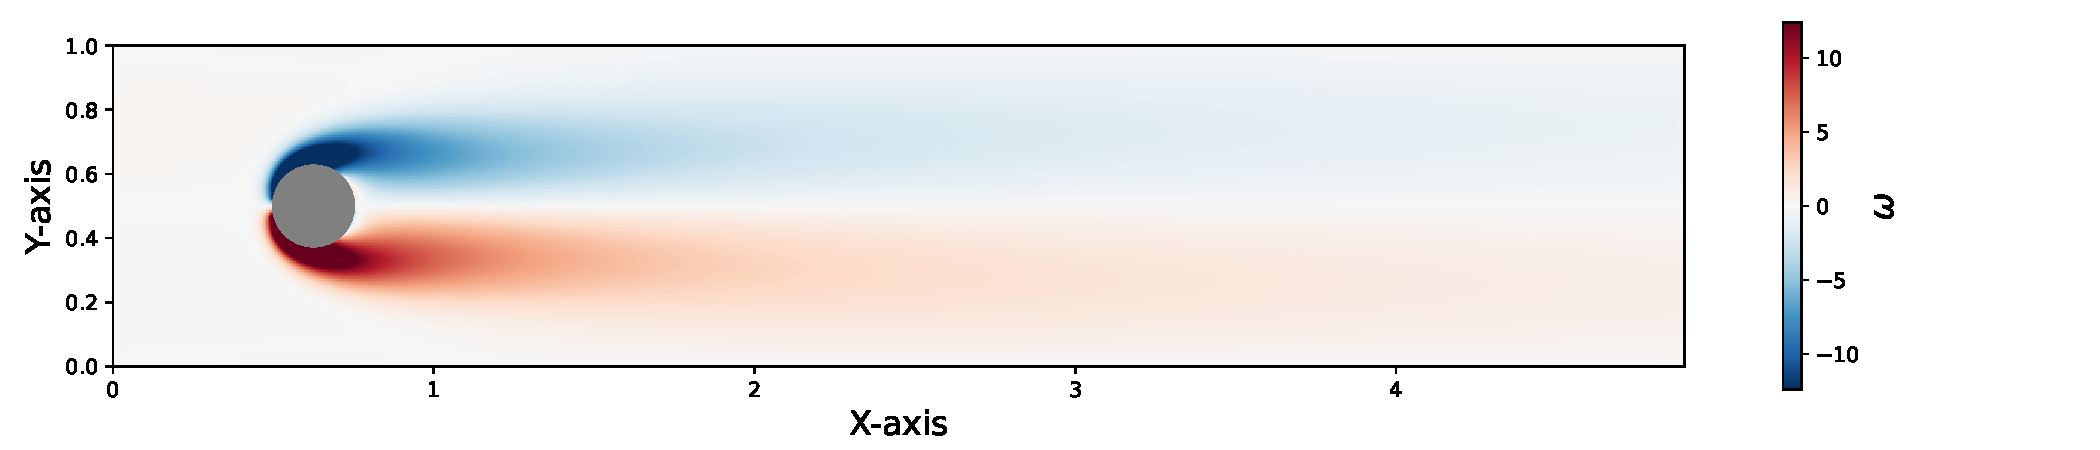
\includegraphics[width=1.1\linewidth]{graphics/numeric/RE100_30_sim.pdf} % Update path accordingly
        \vspace{-0.7cm}
        \caption{Laminar flow at $\Rey = 100$ ($ \Leftrightarrow\, U = 0.006$)}
    \end{figure}
    \vspace{-0.7cm}
    \begin{figure}
        \centering
        \hspace*{0.3cm}
        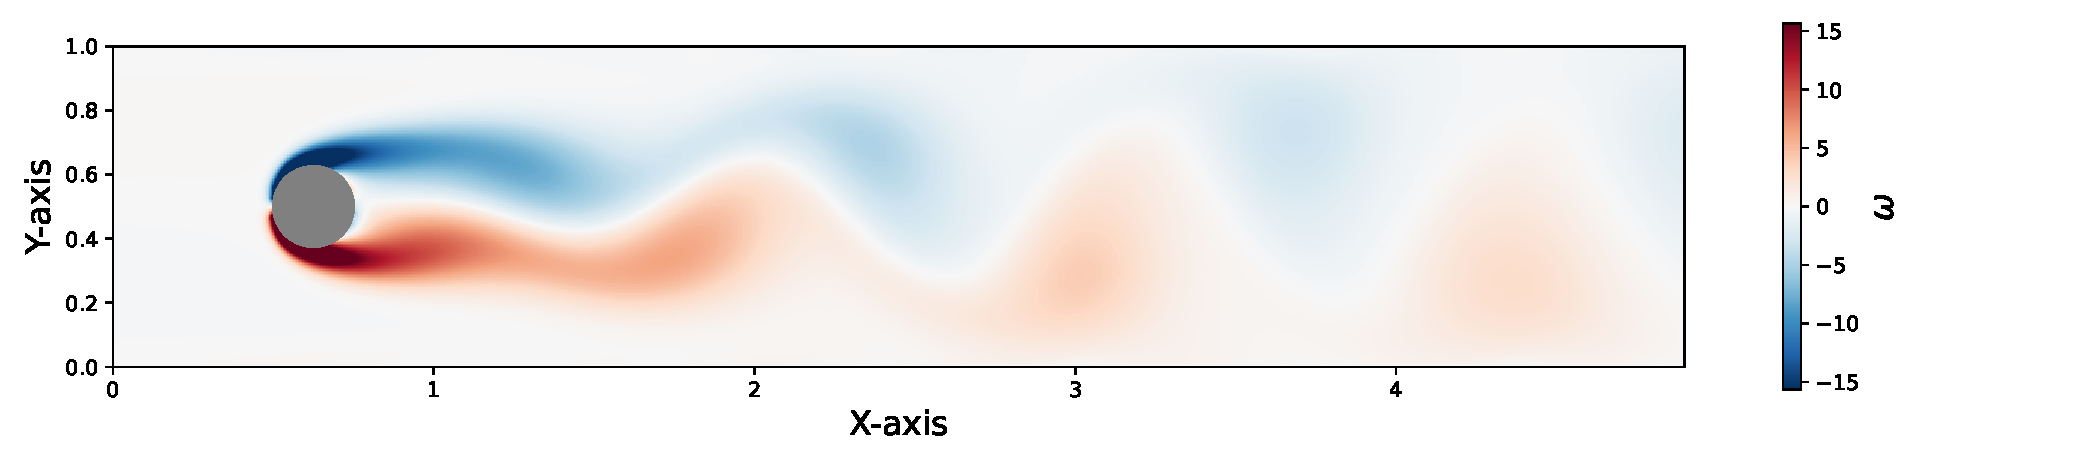
\includegraphics[width=1.1\linewidth]{graphics/numeric/RE190_30_sim.pdf} % Update path accordingly
        \vspace{-0.7cm}
        \caption{Vortex street at critical $\Rey = 190$ ($ \Leftrightarrow\, U = 0.0114$)}
    \end{figure}

\end{frame}

\begin{frame}{Influence of the shape on the flow}
    \begin{figure}
        \centering
        \hspace*{0.3cm}
        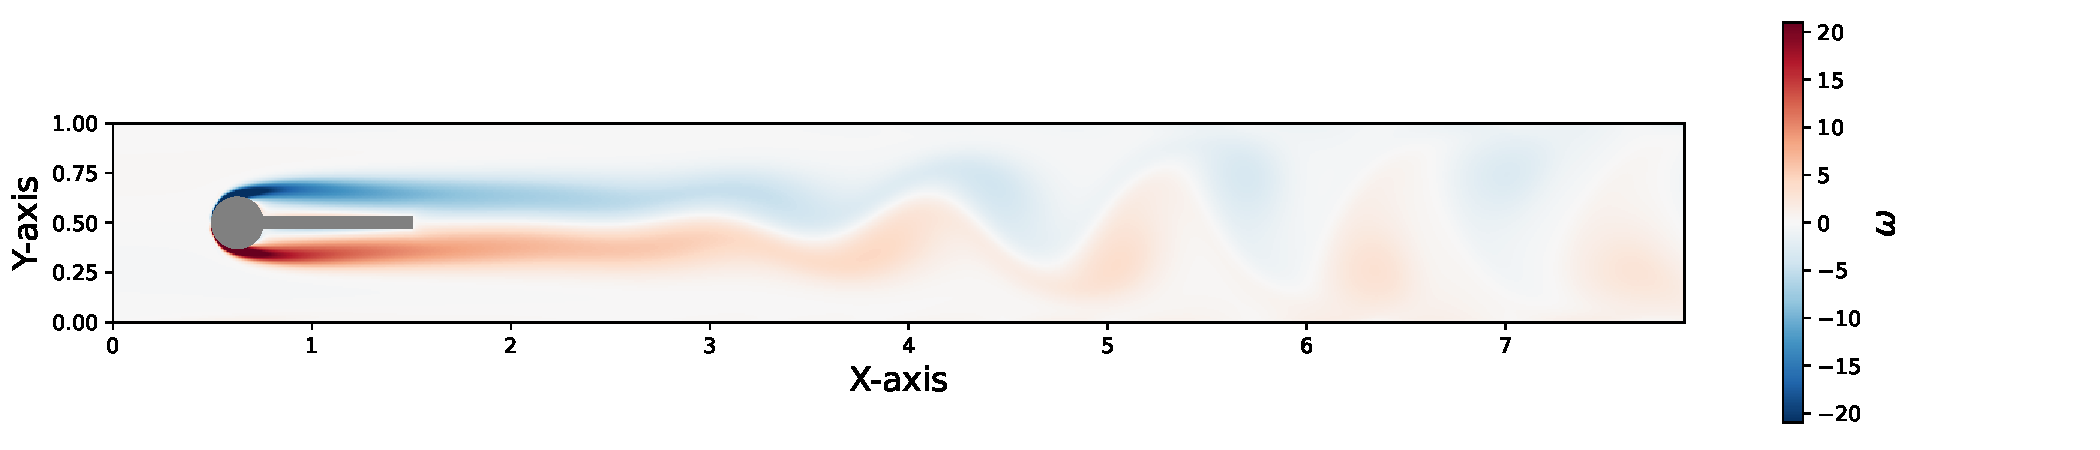
\includegraphics[width=1.1\linewidth]{graphics/numeric/vor_30_circlefin.pdf}
        \vspace{-0.7cm}
        \caption{Flow around circle with fin at $\Rey = 500$ ($ \Leftrightarrow\, U = 0.03012$)}
    \end{figure}
    \textbf{Observation:}
    \begin{itemize}
        \item Fin alters flow, delaying the separation.
        \item Flow transitions at $\Rey \approx 500$, enhancing mixing and vortex complexity.    
    \end{itemize}
\end{frame}

\begin{frame}{Optimized shape: Airfoil}
    %the wing to showcase the influence of the shape
    
    \begin{figure}
        \centering
        \hspace*{0.3cm}
        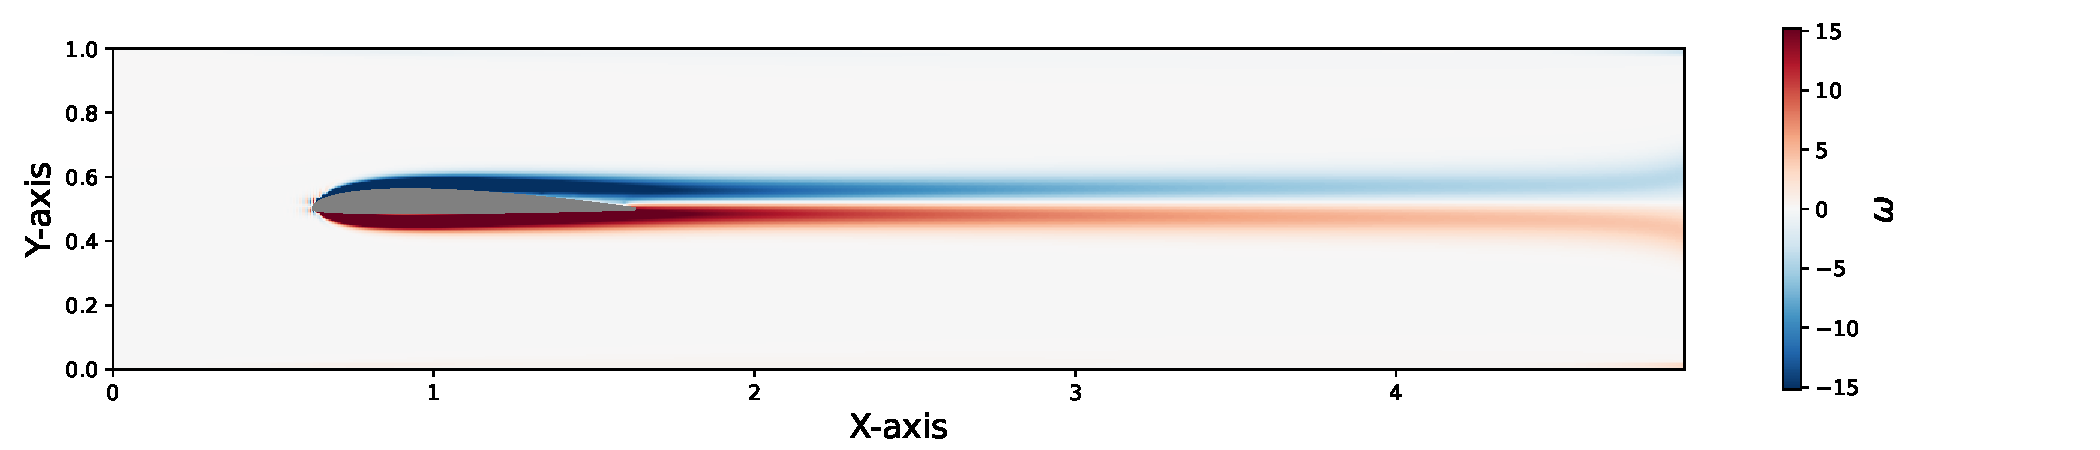
\includegraphics[width=1.1\linewidth]{graphics/numeric/RE3500_30_airfoil.pdf} % Update path accordingly
        \vspace{-0.7cm}
        \caption{Flow with airfoil at $\Rey = 500$ ($ \Leftrightarrow\, U = 0.1076$)}
    \end{figure}
    \vspace{-0.7cm}
    \begin{figure}
        \centering
        \hspace*{0.3cm}
        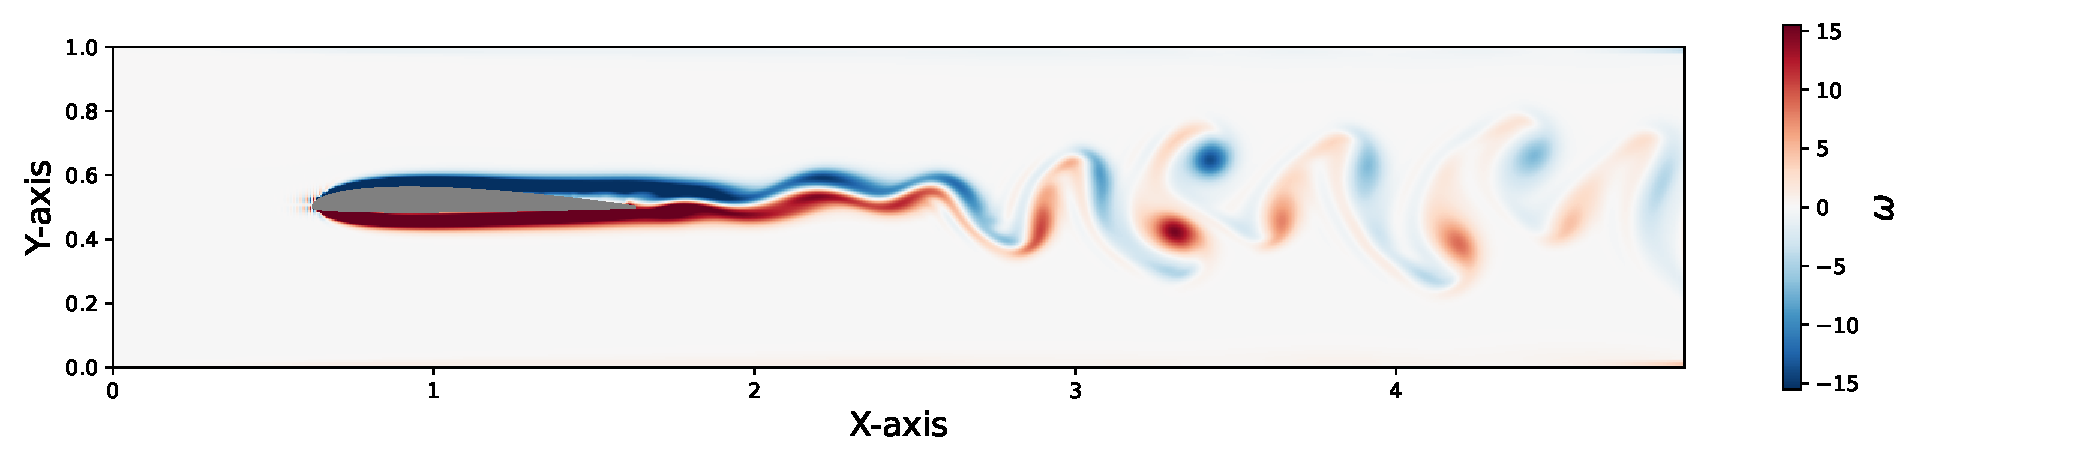
\includegraphics[width=1.1\linewidth]{graphics/numeric/RE5500_30_airfoil.pdf} % Update path accordingly
        \vspace{-0.7cm}
        \caption{Flow with airfoil at $\Rey = 5500$ ($ \Leftrightarrow\, U = 1.1833$)}
    \end{figure}
    \vspace{-0.3cm}
    \textbf{Key Insight:} Airfoil shape minimizes vortex shedding. Streamlined design reduces flow separation and turbulence at higher speeds.
\end{frame}

%#####################################################################################################################################
\section{Conclusion}
\begin{frame}{Conclusion}
    \textbf{Summary:}
    \begin{itemize}
        \item Utilized Chorin's method for numerical analysis of von Kármán vortex street.
        \item Adopted second-order schemes for advection, diffusion, and pressure.
        \item Implemented no-slip conditions for shape-specific flow behavior.
    \end{itemize}
    
    \textbf{Implications:}
    \begin{itemize}
        \item Demonstrated the influence of shape and Reynolds number on flow dynamics.
        \item Identified critical transitions in flow patterns, emphasizing the importance of aerodynamic design.
        \item Showcased the potential for optimizing performance and efficiency in engineering applications.
    \end{itemize}
\end{frame}


%#####################################################################################################################################



\section{References} \subsection{}

\begin{frame}[allowframebreaks]{References}

  \printbibliography[heading=none]

\end{frame}

\begin{frame}
  \begin{center}
    \Large Thank you for your attention!
  \end{center}
\end{frame}


\end{document}

